\chapter{Introduction}
 
Nowadays the usage of the ARM-MCU could be used in every aspect of everyday life.
Additionally, the ARM processor is the number one architecture of choice in 
many market segments.\\ 
This project is based on the development of a bootloaders and its implementation 
inside a network.\\
The usage stm32f4-discovery Board is a prefered and viewed as an "'Allrounder"'
for such a project. The reasoning behind this is the "value for money" and 
user-friendliness. This allows for an easy introduction into the world of ARM
Microcontroller unit programming.\\
The ARM-Cortex-M4-Prozessor found on the STM32f4-discovery board prossesses 
the principel parts shown in the figure below.\\
\section{The Aim}
The aim of the project is to research the feasibility to create a quick, cheap 
and easy to use way of utilizing an STM32 Microcontroller to communicate between 
a user and a remote device.\\
The purpose of the application is meant to be a first step fundamental strategy to 
creating a product for future projects.\\
It is hoped that by way of HTML communication, a fast and light application could 
be used to fulfill the desire of a user to achieve a particular objective such 
as threeway handshake signal to verify a particular device in order to transmit 
information such as codes or messages, using a TCP/IP protocol stake.\\
As it can be demonstrated the different applications could be endless.\\ 

\begin{figure}[ht]
	\centering
	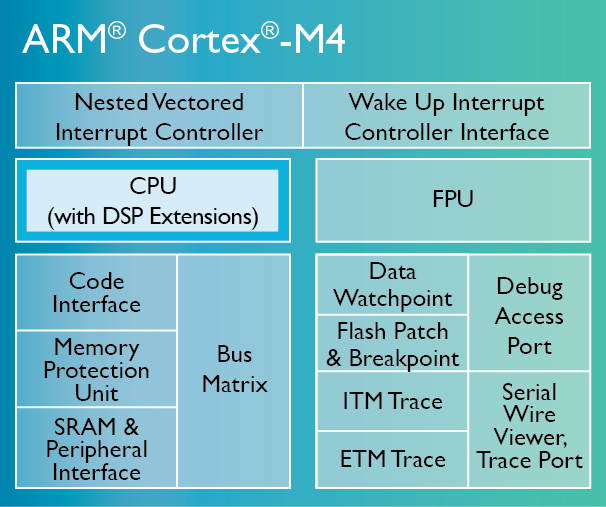
\includegraphics[width=400px, height=300px]{../img/Cortex-M4-chip-diagram-LG.png}
	\caption{Prinzipieller Aufbau}
	\label{m4_prinzip}
\end{figure}

Es wird sp\"ater ein weiteres unterschiedliches Diagram verwendet. Dies ist nicht
falsch, sondern dient der sinngem\"a"sen Darstellung des Prozessors.\\


Zun\"achst soll ein \"Uberblick \"ueber die behandelten Themenschwerpunkte gegeben
 werden 

\section{Bootloader}
The purpose of a Bootloader program is to allow the installation and utilisation 
of any program that could be reloaded. Whereas the program that is currently loaded is also being run.\\
Next it is necessary to initialise the hardware, that would in turn be needed to load the program.\\
The "STM32f407 discovery board" offers three different methodes to boot up the hardware.\\
In order to switch between the three different boot methods, the Boot-Pins BOOT1
and BOOT2 could be set:\\\\
\begin{tabular}{|c|c|l|l|}
\hline \hline
  BOOT1 & BOOT2 & Boot-Mode & Adresse\\ \hline
  x & 0 & Flash Memory (User Flash) & 0x8000\_0000\\
\hline
  0 & 1 & System Memory & 0x1FFF\_F000\\
\hline
 1  & 1 & SRAM & 0x2000\_0000\\
\hline
\end{tabular}\\\\
Der ROM, hier System Memory, beinhaltet den, vom Hersteller, mitgegebenen
 Bootloader.\\
Wie man den Speicher dann belegt ist einem freigestellt. Man muss dann darauf
achten, dass man an die richtige Adresse springt, wenn man das Programm nachgeladen
hat.\\
Als Beispiel-Vorgehensweise kann man sagen, dass die Reihenfolge, nachdem der
Bootloader bereits geladen ist, folgende ist:\\

\begin{enumerate}
\item Verwendete Hardware initialisieren (USB/USART/RCC...)
\item Auf eingehendes Programm warten (wenn sonst keine Aufgabe ansteht)
\item Eingehendes Programm an Adresse XY schreiben.
\item An Adresse XY springen
\end{enumerate}

Das eingegangene Programm ist dann nat\"urlich selbst f\"ur die Initialisierung
der verwendeten Hardware zust\"andig.\\

\section{SWD}
Bei der Entwicklung kam die Serial Wire Debug Technologie zum Einsatz. Hierbei 
handelt es sich um einen Debug-Port, der speziell daf\"ur entwickelt wurde
 um MCU bzw. Projekte mit MCU, bei denen so wenig wie m\"oglich Pins verwendet
 werden sollen. \\
Dieser Port besteht aus den Leitungen folgender Tabelle:\\\\
\begin{tabular}{|c|c|c|p{10cm}|}
\hline \hline
	Pin & Signal & Type & Beschreibung \\ \hline
1 & VTref & Input & This is the target reference voltage. It is used to
 check if the target has power, to create the logic-level reference for
 the input comparators and to control the output logic levels to the target.
 It is normally fed from Vdd of the target board and must not have a series resistor.\\ \hline
7 & SWDIO & I/O & Single bi-directional data pin\\ \hline
9 & SWCLK & Output & Clock signal to target CPU. It is recommended that
 this pin is pulled to a defined state of the target board. Typically
 connected to TCK of target CPU.\\ \hline
13 & SWO & Output & Serial Wire Output trace port. (Optional, not required
for SWD communication)\\ \hline
15 & RESET & I/O & Target CPU reset signal. Typically connected to the
 RESET pin of the target CPU, which is typically called "nRST", "nRESET"
 or "RESET".\\ \hline
19 & 5V-Supply & Output & This pin is used to supply power to some eval boards.
Not all JLinks supply power on this pin, only the KS (Kickstart) versions.
Typically left open on target hardware.\\ \hline
\end{tabular}\\\\

Die anderen Leitungen des bisherigen 20-poligen Anschlussen wurden weggelassen,
weil sie entweder f\"ur SWD uinteressant sind oder sie auf GND gelegt sind. Egal
was davon zutrifft, sie haben keinen Einfluss auf die SWD-Kommunikation.

Es ist eine neue, sehr interessante Weise zu debuggen. Bisher war JTAG das
Debugger-Interface. 
Die Vorteile dieser Technologie sind (frei von der ARM-Website \"ubersetzt):

\begin{itemize}
\item Nur 2 Pins werden belegt
\item JTAG TAP controller kompatibel
\item Erlaubt dem Debugger ein weiterer AMBA-Bus-Master zu werden um auf
Register / Speicher zuzugreifen.
\item High Datarates - 4Mbytes/sec @50MHz
\item Low Power - keine zus\"atzlichen Versorgungsspannung
\item gute "'built in"' Fehler-Erkennung
\item Schutz vor Fehlern bei Kontaktverlust
\end{itemize}  

\section{startup}
 - stack, program counter, interrupt, vector table, initial system clock

\section{CMSIS}
Der ARM Cortex Microcontroller Software Interface Standard ist eine 
H\"andlerunabh\"angige Abstraktionsschicht f\"ur die Cortex-M Prozessoren.\\
Dabei ist CMSIS unterteilt in:
\begin{itemize}
\item CMSIS-CORE - API zum Zugriff auf den Prozessorkern sowie Perepherie-Register.
\item CMSIS-Driver - Generischer Zugriff auf Perepherie f\"ur die Middleware
			(reusability).
\item CMSIS-DSP - DSP Bibliothek mit \"uber 60 Funktionen
\item CMSIS-RTOS API - Standardisiertes (RTOS kompatibel)
\item CMSIS-Pack - Beschreibung der wichtigen Bestandteile (Nutzersicht)
\item CMSIS-SVD - Beschreibung der wichtigen Bestandteile (Systemsicht)
\item CMSIS-DAP - Debug Access Port
\end{itemize}

Zusammengefasst erlaubt CMSIS einheitliche und simple Software Schnittstelle
zu Prozessor und die Perepherie, sowie Echtzeit OS (RTOS) und Middleware.

\section{Nested Vectored Interrupt Controller}
Der NVIC bietet die M\"oglichkeit gewisse Interrupts zu konfigurieren
(Priorit\"at, aktiviert, deaktiviert...). \\
Neben vorgegebenen Interrupts sind hier auch die Implementierungsabh\"angigen
Interrupts konfigurierbar. Da die ersten 15 Interrupts vorgegeben sind, k\"onnen
die implementierten Interrupts in der Anzahl von 0 bis 240 reichen.

\section{Unterschiede}
GNU, KEIL iar

\section{Netzwerk}
was sollte zum besseren verstehen hier einen platz finden.
